\documentclass[a4paper,twoside,kulak]{kulakreport}



\usepackage[dutch]{babel}
\usepackage{hyperref}
\usepackage{graphicx}
\usepackage{flafter}
\usepackage{amsmath, amssymb, amsthm}
\usepackage{siunitx}
\usepackage{pdfpages}
\usepackage{subfiles}
\usepackage{wrapfig}
\usepackage{float}
\usepackage{url}
\usepackage{translator}
\usepackage{pdfpages}

\uselanguage{Dutch}
\languagepath{Dutch}
\providetranslation[to=Dutch]{Figure}{Figuur}



\faculty{Groep Wetenschappen \& Technologie}
\group{\texttt{X0B54a} -- Probleemoplossen en ontwerpen, deel 2}
\title{Smart City}
\subtitle{Tussentijds verslag}
\author{Team 4: Team R2D2}
%\emailaddress{}
\institute{Matthijs Deforche, Karl Van Holder, Thomas Varheust, Kobe De Weerdt, Yaron Verhulst}
\date{Academiejaar 2020 -- 2021}
\address{\textbf{\theauthor}\\
	Groep Wetenschap \& Technologie \\
	KU Leuven Kulak           \\
	Etienne Sabbelaan 53, 8500 Kortrijk
}

\begin{document}
	\titlepage
	
	\chapter*{Abstract}
	
	\renewcommand*\contentsname{Inhoud}
	\tableofcontents
	
	\chapter{lijsten van tabellen, figuren en grafieken}
	
	\chapter*{Inleiding}
	Wij zijn vijf studenten ingenieurswetenschappen in het eerste jaar aan de Katholieke Universiteit Leuven Campus Kulak Kortrijk.
	Het vak P\&O 1 en de andere vakken van het eerste semester hebben ons de nodige kennis gegeven om het vak P\&O 2 aan te vatten. 
	De opzet van de teamopdracht dit semester is een zelfrijdend wagentje te ontwerpen en te bouwen dat uiteindelijk zelfstandig door een modelstad zal moeten rijden. Het wagentje moet niet alleen kunnen rijden, ook moet het obstakels zoals tegenliggers en voorgangers kunnen ontwijken. Het wagentje zal kruispunten en verkeerslichten correct moeten kunnen interpreteren en zal er gepast op moeten reageren. Dit zou allemaal foutloos moeten gebeuren. Het ontwerpen en het bouwen van het wagentje kan met behulp van een virtueel budget, een interface LabView om met het wagentje te kunnen communiceren, een CAD-programma om onze wagen te 3D-modelleren enz. 
	Tijdens het ontwerpen, zullen we ook een persoonlijke touch aan het wagentje geven. 
	
	%%hoofdtekst
	\chapter{methodologie}
	
	
	
	\chapter{Planning}
	\section{Klantenvereisten}
	Voor de planning van onze teamopdracht hebben we enkele tools gebruikt die we kunnen gebruiken. Eerst en vooral hebben we de klantenvereisten opgesteld. We kregen een opdracht mee met daarin de informatie over wat er allemaal bereikt moet worden op het einde van het project. Deze hebben we per categorie samengebundeld om zo een algemeen overzicht te krijgen van wat er verwacht wordt. 
	\section{Ontwerpspecificaties}Aan de hand van deze klantenvereisten hebben we de ontwerpspecificaties samengesteld. Een klantenvereiste is eerder algemeen terwijl de ontwerpspecificaties veel gedetailleerder zijn. Dit geeft ons een duidelijker beeld van de opdracht. 
	\section{Teamverantwoordelijkheden}Omdat de teamopdracht goede planning vraagt en een goede werkverdeling hebben we teamverantwoordelijken aangesteld. Per categorie zoals programmeren, Solid Edge.. zijn er studenten verantwoordelijk gesteld. 
	\section{Takenstructuur}Om het werk te verdelen onder elkaar hebben we een takenstructuur gemaakt. Deze bevat alle deeltaken die nodig zijn om ons project tot een goed einde te brengen. De deeltaken zijn verdeeld onder een samenvattende hoofdcategorie. Bijvoorbeeld bij de categorie Solid Edge is er een deeltaak 'wiel modelleren'. 
	\section{Gantt-grafiek \& Teamkalender} Nu we de verschillende deeltaken hebben opgesteld is het mogelijk om deze in te plannen. We hebben de deeltaken genummerd en een teamkalender opgesteld om te plannen wanneer een deeltaak afgewerkt moet zijn. Het nummer van de deeltaak wordt bij de week/dag geplaatst wanneer het af moet zijn. Een teamkalender duidt echter niet aan hoeveel tijd het in beslag zal nemen. Daarom hebben we een bijhorende Gantt-grafiek gemaakt. Deze toont per deeltaak hoeveel tijd we eraan zullen besteden. Het is ook handig om aan te tonen wanneer je kan beginnen aan een deeltaak waarbij eerst een andere deeltaak moet afgewerkt worden. Dit kan met pijlen worden aangetoond en dit is mogelijk in de Gantt-grafiek. 
	
	\chapter{Ontwerp}
	\section{Onderdelen}
	We kozen voor de NI Myrio@-microcontroller omdat deze het simpelste is en voor de aard van de opdracht voor ons het efficiëntste leek. Bovendien hebben we via de NI Myrio altijd een handige visualisatie van het programma en kunnen we gebruik maken van de analoge afstandssensor die met een bereik van 10 to 80 centimeter de meest geschikte afstandssensor is.
	Door deze keuze kunnen we voor de andere sensoren enkel de analoge versie gebruiken. Aangezien de NI Myrio een @power input nodig heeft van 6-16 Volt, kan de powerbank niet gebruikt worden. Door 2 Lithium-ion @batterijen van @$3,6$ Volt te kiezen en deze in serie te schakelen is het wel mogelijk om een geschikte power-input te verkrijgen.
	Als persoonlijke touch kozen we om geen makerbeams te gebruiken. Hierdoor leek het ons het beste om een groot chassis te hebben. We kozen het rechthoekig zwart boven het universeel chassis omdat ze redelijk gelijkaardig zijn maar het universeel chassis 50 eenheden meer kost. Om dit chassis stabiel te maken kozen we ervoor om de ball caster te gebruiken samen met 2 @aangedreven wielen. Als wiel kozen we voor de wielen met een breedte van 8 millimeter en diameter van 60 millimeter, deze zijn de grootste en kunnen samen met de spacers van de ball caster ervoor zorgen dat het chassis perfect horizontaal ligt. Als aandrijving hadden we de voorkeur voor de "Micro Metal Gear Motor 50:1 HP". Deze heeft een 3 millimeter as, wat compatibel is met onze gekozen wielen en heeft een gemiddeld vermogen om de wagen te doen stoppen en opnieuw te versnellen. Omdat deze motoren niet meer beschikbaar waren wanneer wij onze bestelling konden plaatsen kozen we voor de "Micro Metal Gear Motor 100:1 HP", deze is redelijk gelijkaardig maar heeft een ander @vermogen. Samen met deze motoren kozen we 2 motorbeugels om de motoren aan het chassis te kunnen bevestigen en de "Dual Drive DRV8833" zodat we beide motoren tegelijk kunnen aansturen.
	Om eerst de wagen te testen voor we gaan solderen op de printplaat kozen we nog een breadbord, aangezien we maar 3 sensoren en 2 motoren hadden kozen we voor het kleinere formaat omdat dit ons minder budget kost.  
	
	\section{budget}
	
	
	\chapter{Resultaten}
	
	\chapter{Discussie}
	%%besluit
	\chapter{Besluit}
	
	
	%%besluit
	
	
	%%referenties
	\bibliography{bibliografie_verslag.bib}
	\bibliographystyle{unsrt}
	
	
	
	%%Bijlagen
	\includepdf{Team4-Ontwerpspecificaties.pdf}
	\includepdf[pages = 2]{Team4-Ontwerpspecificaties.pdf}
	\includepdf[pages = 3]{Team4-Ontwerpspecificaties.pdf}
	
	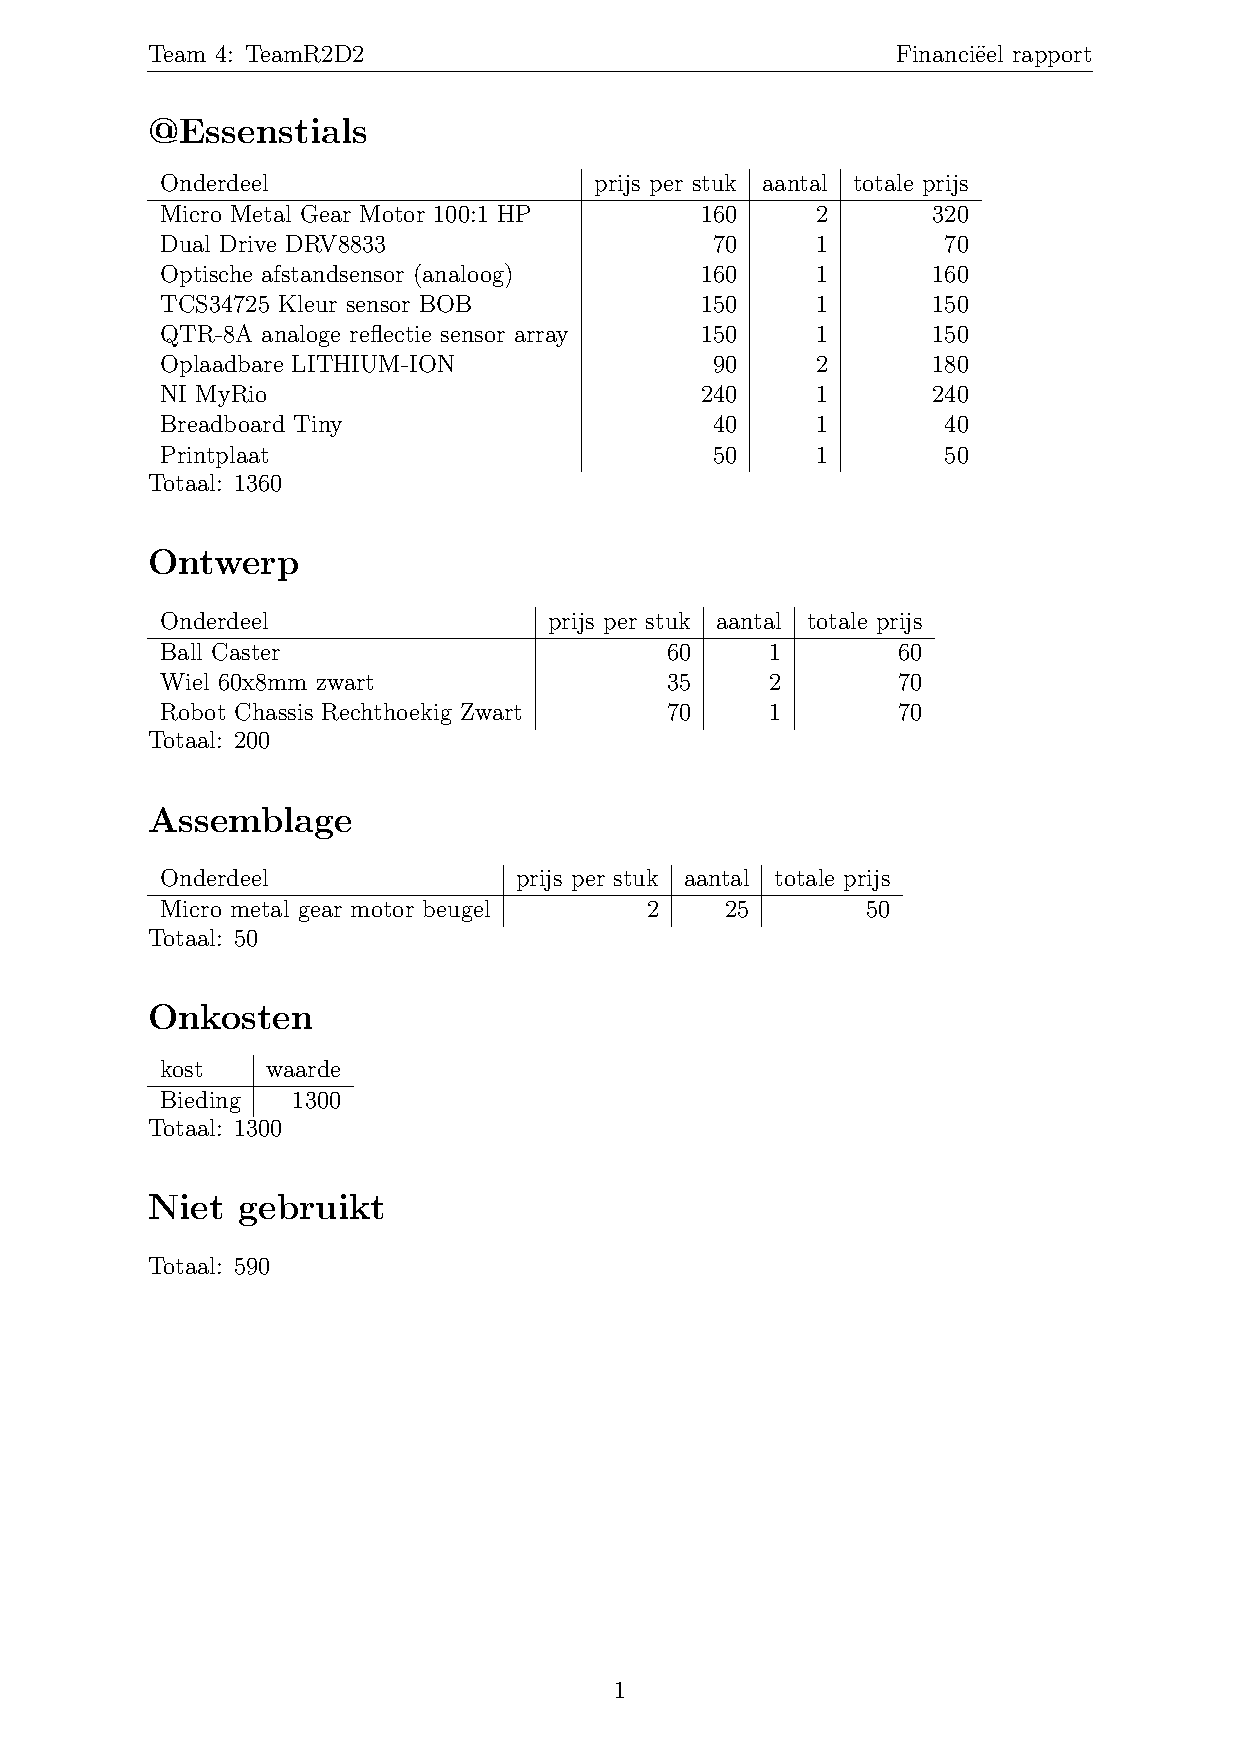
\includepdf{financieelRapport.pdf}
	
	
	
\end{document}